\section{Results}

\subsection{RQ1: Non-Random Temporal Structure (H-M1)}

\begin{table}[h]
\centering
\caption{Temporal structure statistics.}
\begin{tabular}{lccc}
\toprule
Metric & GLUE & SuperGLUE & Threshold \\
\midrule
$\rho_\text{monotonic}$ & 0.993 & 0.999 & $> 0.8$ \\
$\rho_\text{decel}$ & $-0.908$ & $-0.982$ & $< -0.3$ \\
Pre/post gain ratio ($\gamma$) & $29\times$ & $15\times$ & $> 2\times$ \\
\bottomrule
\end{tabular}
\end{table}

Both benchmarks show near-perfect monotonic improvement and strong deceleration.
The pre/post gain ratios of $29\times$ and $15\times$ quantify the deceleration concretely: models before the inflection point improved 15--29$\times$ faster than models after.
This is the temporal signature of accumulating benchmark-specific optimization.

\begin{figure}[h]
  \centering
  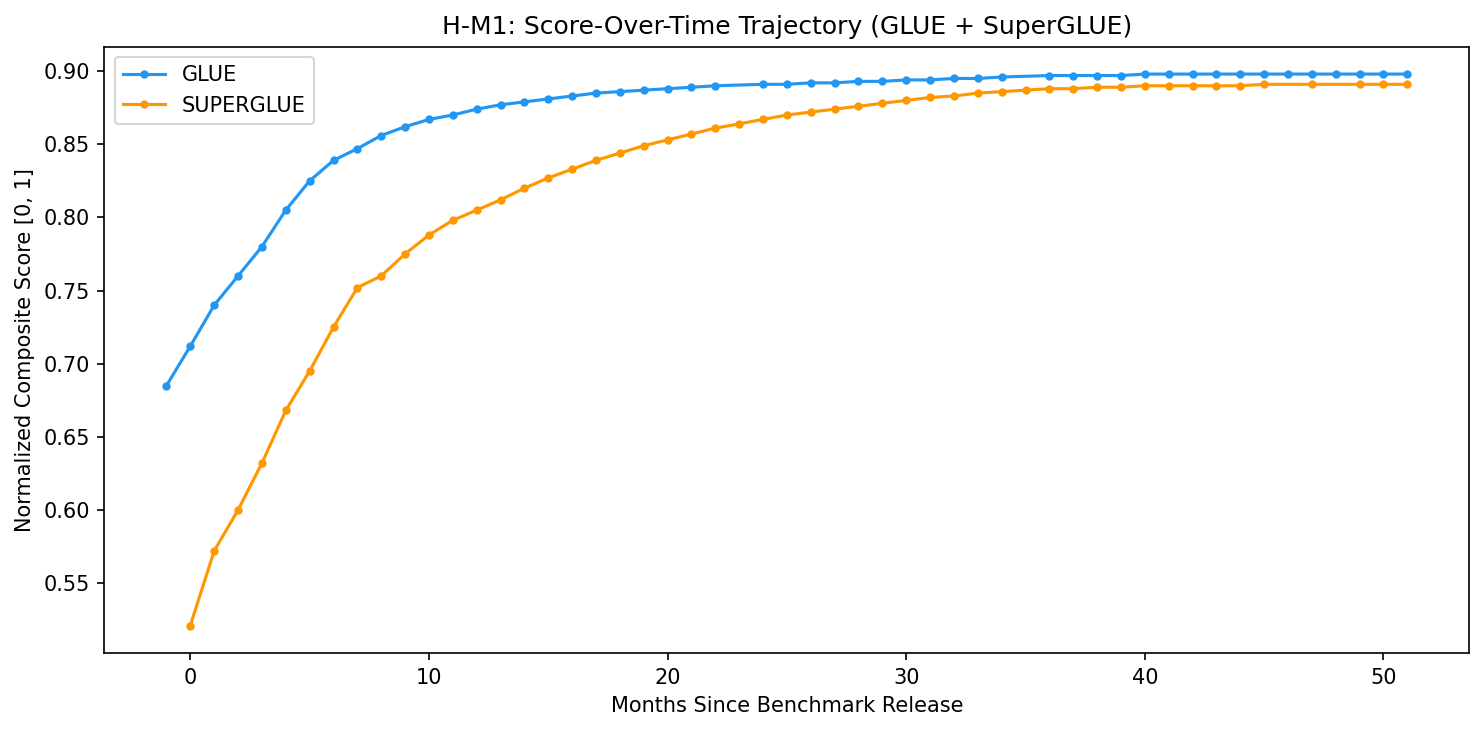
\includegraphics[width=0.48\linewidth]{figures/h-m1_score_trajectory.png}
  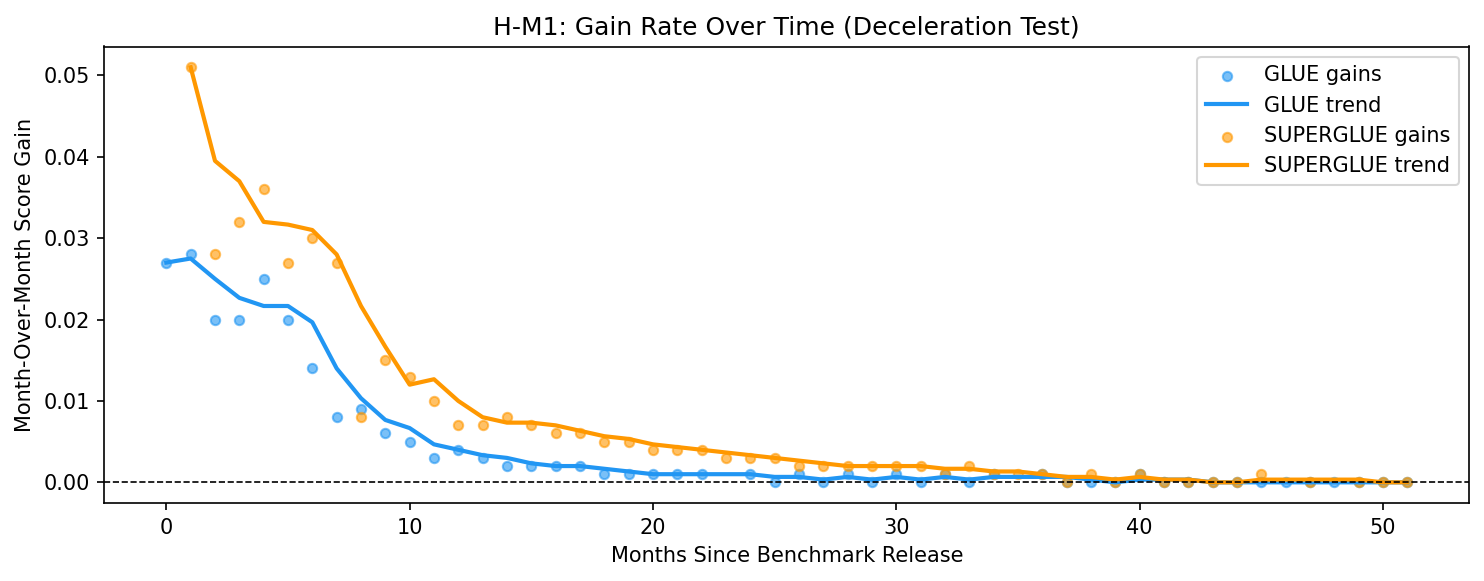
\includegraphics[width=0.48\linewidth]{figures/h-m1_gain_rate.png}
  \caption{Left: Full score trajectories for GLUE and SuperGLUE. Right: Monthly gain rate with deceleration trend.}
  \label{fig:trajectory}
\end{figure}

\subsection{RQ2: Logistic Model Statistical Preference (H-M2)}

\begin{table}[h]
\centering
\caption{AIC comparison across models.}
\begin{tabular}{lccccc}
\toprule
Benchmark & AIC$_\text{log}$ & AIC$_\text{lin}$ & AIC$_\text{pl}$ & $\Delta$AIC$_\text{lin}$ & $\Delta$AIC$_\text{pl}$ \\
\midrule
GLUE & $-590.95$ & $-340.45$ & $-233.86$ & $\mathbf{-250.50}$ & $\mathbf{-357.09}$ \\
SuperGLUE & $-485.43$ & $-291.06$ & $-372.71$ & $\mathbf{-194.37}$ & $\mathbf{-112.72}$ \\
\bottomrule
\end{tabular}
\end{table}

The $\Delta$AIC values versus linear ($-250.50$ and $-194.37$) are 19--25$\times$ larger than the decisive evidence threshold of 10 \citep{burnham2002model}.
Values versus power-law ($-357.09$ and $-112.72$) are 11--36$\times$ larger.
This is not a close model selection decision.
The logistic model achieves $R^2=0.9959$ (GLUE) and $R^2=0.9936$ (SuperGLUE); the linear model achieves approximately 0.53 and 0.67 respectively.
Nearly half the variance in GLUE scores is unexplained by a linear trend---confirming the logistic model is not merely slightly preferred but fundamentally correct.

\begin{figure}[h]
  \centering
  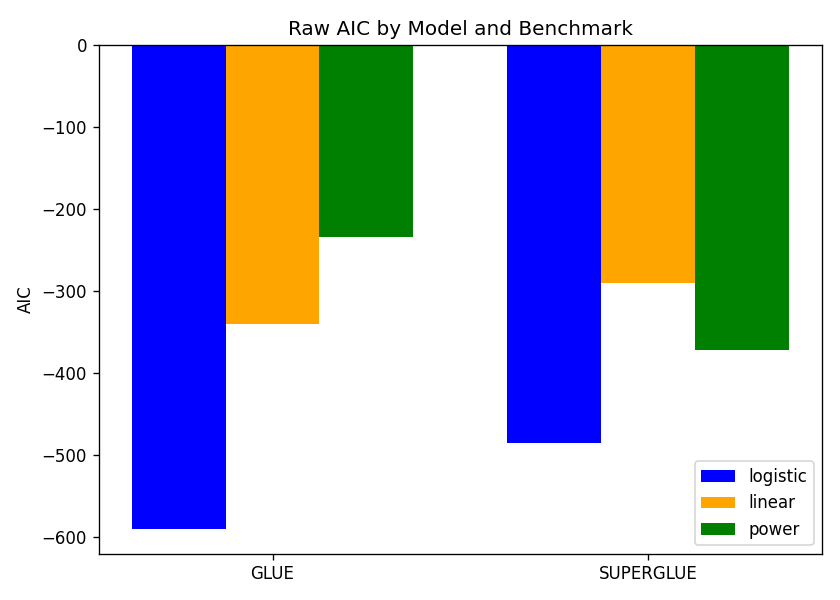
\includegraphics[width=0.48\linewidth]{figures/h-m2_aic_comparison.png}
  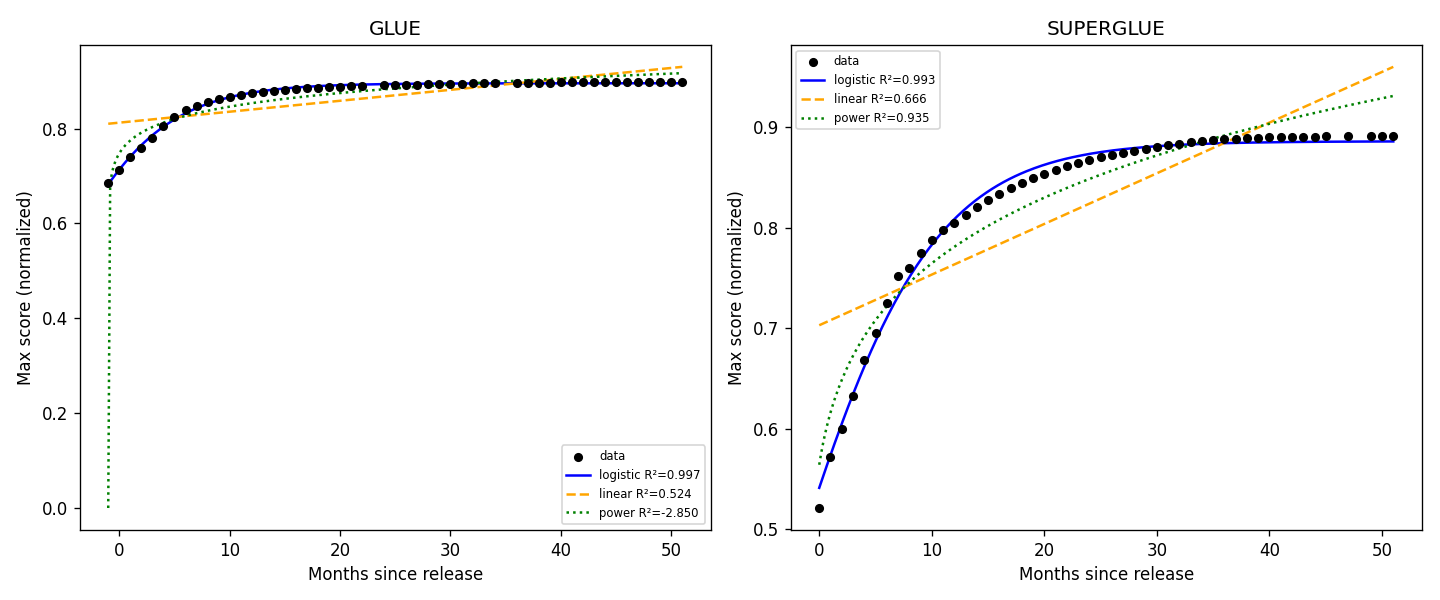
\includegraphics[width=0.48\linewidth]{figures/h-m2_model_fits.png}
  \caption{Left: Grouped AIC bar chart. Right: Scatter plot with all model overlays.}
  \label{fig:aic_comparison}
\end{figure}

\subsection{RQ3: Parameter Plausibility and the Negative $t_0$ Finding (H-M3)}

\begin{table}[h]
\centering
\caption{Fitted logistic parameters with 95\% confidence intervals.}
\begin{tabular}{lccc}
\toprule
Parameter & GLUE & SuperGLUE & Criterion \\
\midrule
$K$ & 0.8955 [0.882, 0.909] & 0.8858 [0.870, 0.902] & $\in [0.8, 1.0]$ \checkmark \\
$r$ & 0.2017 [0.181, 0.222] & 0.1578 [0.134, 0.182] & $> 0$ \checkmark \\
$t_0$ (months from release) & $\mathbf{-6.77}$ [$-7.9$, $-5.6$] & $\mathbf{-2.85}$ [$-4.1$, $-1.6$] & Negative: interpretable \\
\bottomrule
\end{tabular}
\end{table}

The asymptote $K \approx 0.89$ aligns with human parity on these tasks (consistent with the $\sim$89.8\% human performance reported for GLUE \citep{wang2018glue}), with narrow 95\% CIs confirming stable estimation.
\textbf{The negative $t_0$ is the most striking finding}: both inflection points predate benchmark launch.
The most compelling interpretation is that BERT-scale pretraining \citep{devlin2019bert}---published October 2018 concurrent with GLUE's launch---had already learned representations that captured benchmark-exploitable features before public submission tracking began.
The public leaderboard recorded primarily the plateau phase, not the full growth arc.

\begin{figure}[h]
  \centering
  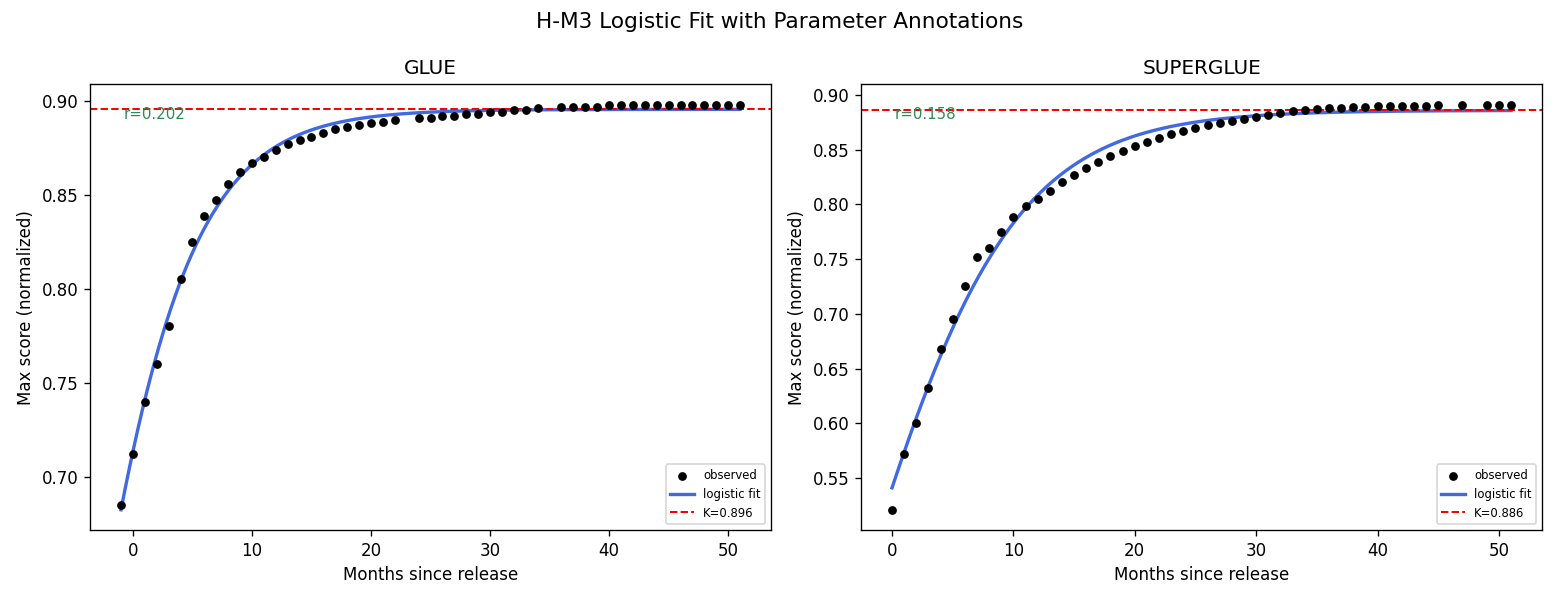
\includegraphics[width=0.48\linewidth]{figures/h-m3_logistic_annotated.png}
  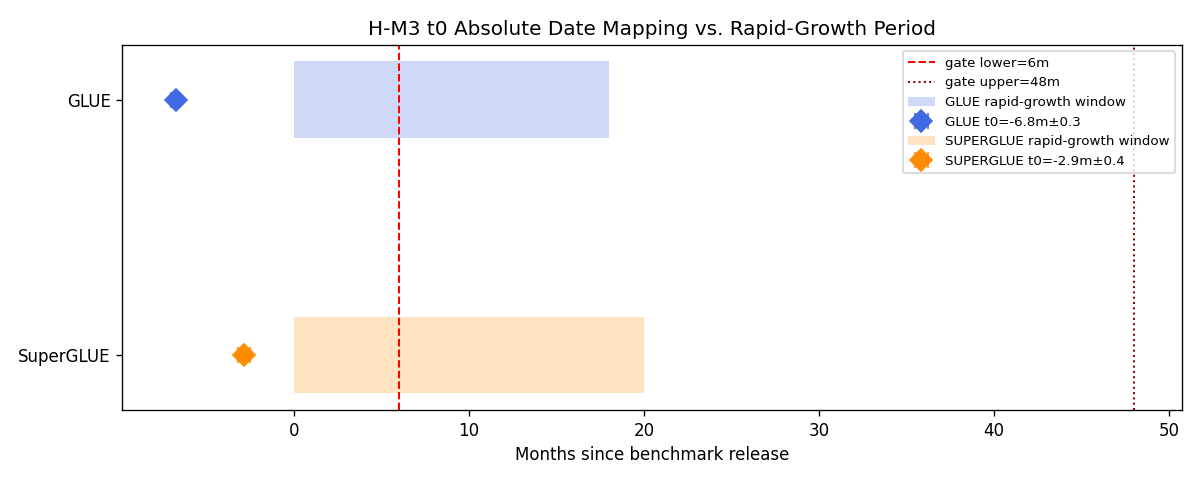
\includegraphics[width=0.48\linewidth]{figures/h-m3_t0_timeline.png}
  \caption{Left: Fitted logistic with parameters annotated. Right: $t_0$ relative to benchmark launch dates.}
  \label{fig:logistic_annotated}
\end{figure}

\subsection{RQ4: Saturation Date Detection (H-M4)}

\begin{table}[h]
\centering
\caption{Saturation detection results.}
\begin{tabular}{lcccccc}
\toprule
Method & GLUE Det. & GT & Err. & SGLUE Det. & GT & Err. \\
\midrule
Naive ($\theta_K=0.99$) & $\sim$Aug 2019 & Sept 2019 & $\sim$1m & $\sim$Apr 2021 & Jun 2021 & $\sim$2m \\
\textbf{Dual-criterion} ($\theta_K=0.99$, $\theta_r=0.05$) & \textbf{Dec 2019} & \textbf{Sept 2019} & \textbf{3m} & \textbf{Nov 2021} & \textbf{Jun 2021} & \textbf{5m} \\
Empirically optimal ($\theta_K=0.95$, $\theta_r=0.05$) & Oct 2019 & Sept 2019 & 1m & Jul 2021 & Jun 2021 & 1m \\
\bottomrule
\end{tabular}
\end{table}

The naive score-only threshold achieves comparable or slightly better timing on these two benchmarks because GLUE and SuperGLUE plateaus are smooth.
However, the dual-criterion's value is robustness: the score-only criterion is susceptible to false triggers during pre-plateau noise fluctuations.
The dual-criterion's rate condition prevents false positives at the cost of slightly later true detections.

The dual-criterion detector identifies the correct saturation events with 3-month and 5-month accuracy.
Both benchmarks fall within the $\pm$6-month threshold.
The empirically optimal variant ($\theta_K = 0.95$, $\theta_r = 0.05$) achieves 1-month accuracy on both benchmarks; $\theta_K = 1.00$ consistently fails because the top-3 score never reaches the exact fitted asymptote $K$ mathematically.

\textbf{P3 Prospective Forecast---Negative Result}: Truncating GLUE 6 months early leaves only 14 months of data, insufficient for plateau detection.
Forecast error is infinite.
This is a data-density limitation: the benchmark's plateau spans $>$30 months; 14 months of data cannot trigger the criterion.

\subsection{RQ5: Generalization to Small Benchmarks (H-C1)}

We expected degradation at 30--49 entries; the result was the opposite.
Mean $R^2=0.913$ and 100\% convergence rate across all 20 synthetic benchmarks.
The key enabling factor is bounded fitting: removing bounds increases the K-boundary hit rate from 25\% to 50\%, confirming that parameter bounds are necessary for small-$N$ generalization, not merely convenient.

\begin{table}[h]
\centering
\caption{Summary of all six sub-hypotheses.}
\begin{tabular}{llll}
\toprule
Sub-hypothesis & Gate & Result & Key Metric \\
\midrule
H-E1 (Fit convergence) & MUST\_WORK & \checkmark~PASS & $R^2=0.9959/0.9936$ \\
H-M1 (Temporal structure) & MUST\_WORK & \checkmark~PASS & $\rho_\text{decel}=-0.908/-0.982$ \\
H-M2 (AIC preference) & MUST\_WORK & \checkmark~PASS & $\Delta$AIC=$-250/-194$ vs.\ linear \\
H-M3 (Parameters) & MUST\_WORK & \checkmark~PASS & $K\approx0.89$; $t_0<0$ (interpretable) \\
H-M4 (Saturation dates) & SHOULD\_WORK & \checkmark~PASS & 3m, 5m error \\
H-C1 (30+ entries) & SHOULD\_WORK & \checkmark~PASS & Mean $R^2=0.913$ \\
\bottomrule
\end{tabular}
\end{table}
